\chapter{鮮度の表現方法の考察}
\label{chap:verification}

本章では,視覚化システムで採用する鮮度の表現方法を考察する.

実際の検索結果一覧画面をキャプチャし,画像編集ソフトで様々な加工を施すことで視覚化方法の試作を行った.

またそれらを比較検討し,各表現方法を評価した.

\newpage

\section{準備}

評価する全ての表現方法に関して図\ref{fig:ver-base}をベースに加工する.

\begin{figure}[htbp]
  \begin{center}
    \fbox{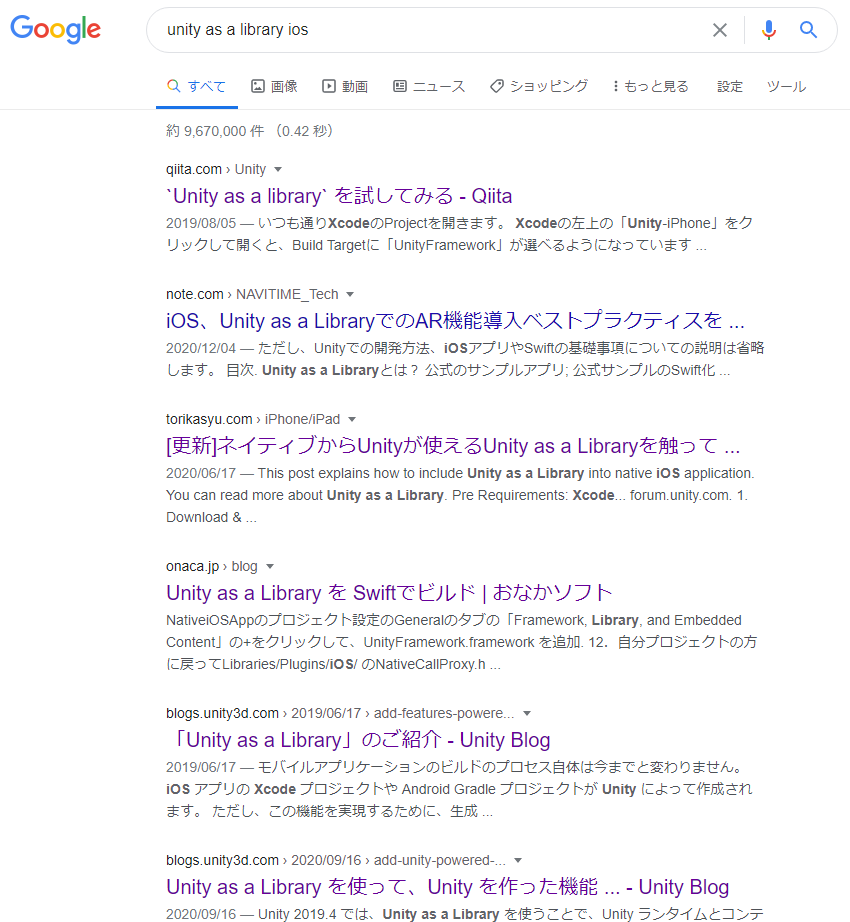
\includegraphics[width=60mm]{images/base.png}}
  \end{center}
  \caption{視覚化前の検索結果一覧画面}
  \label{fig:ver-base}
\end{figure}

各表現方法は類似した系統ごとに分類して紹介する.以下に系統を示す.

\begin{description}[style=sameline]
  \item[テクスチャによる表現方法] テクスチャ画像を背景に適応する方法
  \item[色による変化] 背景色や文字色を変更する方法
  \item[文字の消失による変化] 文字の存在感を薄くしたりなくしたりする方法
  \item[フォントによる変化] 使用されるフォントを変更する方法
\end{description}

\section{試作}

\subsection{テクスチャによる表現方法}
\label{sec:ver-texture}

\subsubsection{紙の経年劣化}
\label{subsec:ver-tex-sheet}

紙は時間が経つと黄ばみやシミができる.そういった変化を参考に,情報の鮮度に応じた紙のテクスチャを使用する.

\begin{figure}[htbp]
  \begin{minipage}{0.5\hsize}
    \begin{center}
      \fbox{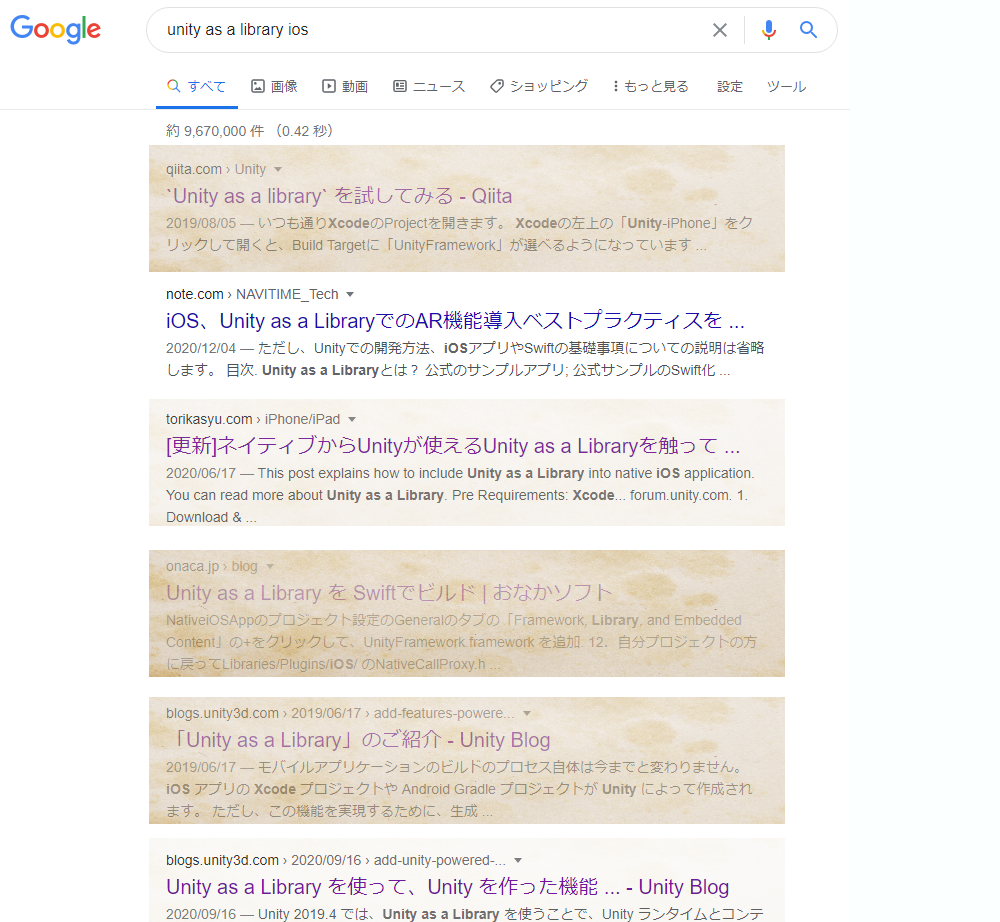
\includegraphics[width=60mm]{images/sheet-degradation1.png}}
    \end{center}
    \caption{紙の経年劣化をイメージした視覚化1}
    \label{fig:ver-sheet1}
  \end{minipage}
  \begin{minipage}{0.5\hsize}
    \begin{center}
      \fbox{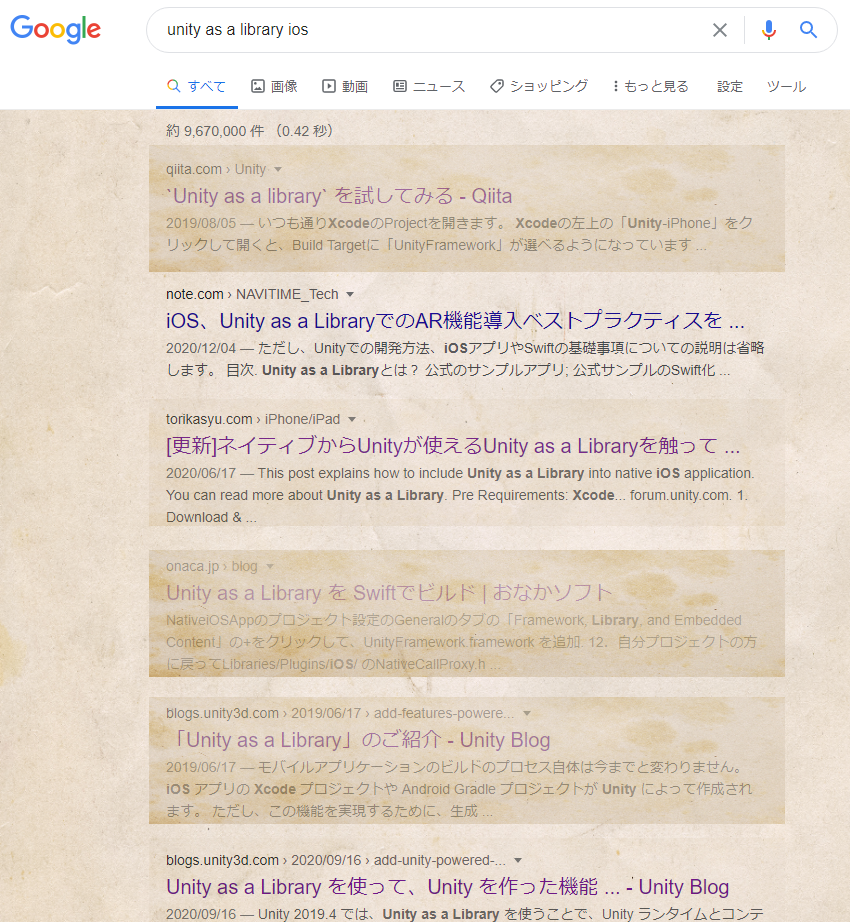
\includegraphics[width=60mm]{images/sheet-degradation2.png}}
    \end{center}
    \caption{紙の経年劣化をイメージした視覚化2}
    \label{fig:ver-sheet2}
  \end{minipage}
\end{figure}

図\ref{fig:ver-sheet1}は,各検索結果ごとに背景に劣化した紙のテクスチャを設定し,それぞれの公開日を参考にして不透明度を調整している.

図\ref{fig:ver-sheet2}は,図\ref{fig:ver-sheet1}に加えて,劣化した紙のテクスチャがなじむように画面全体に紙のテクスチャを適用している.

家や図書館などで古い本を見た経験がある人ならば,紙の時間経過による劣化は古さを連想しやすいため,各情報の鮮度が分かりやすい.

また,図\ref{fig:ver-sheet1}に比べて図\ref{fig:ver-sheet2}は,画面全体にも紙のテクスチャを設定しているため劣化した紙のテクスチャが悪目立ちせず馴染んでいる.

\subsubsection{金属のさび}
\label{subsec:ver-tex-russet}

金属は雨風にさらされてさびが発生するため,時間経過による劣化が簡単に見て取れる.これを参考に情報の鮮度に応じた錆びた金属のテクスチャを使用する.

\begin{figure}[htbp]
  \begin{minipage}{0.5\hsize}
    \begin{center}
      \fbox{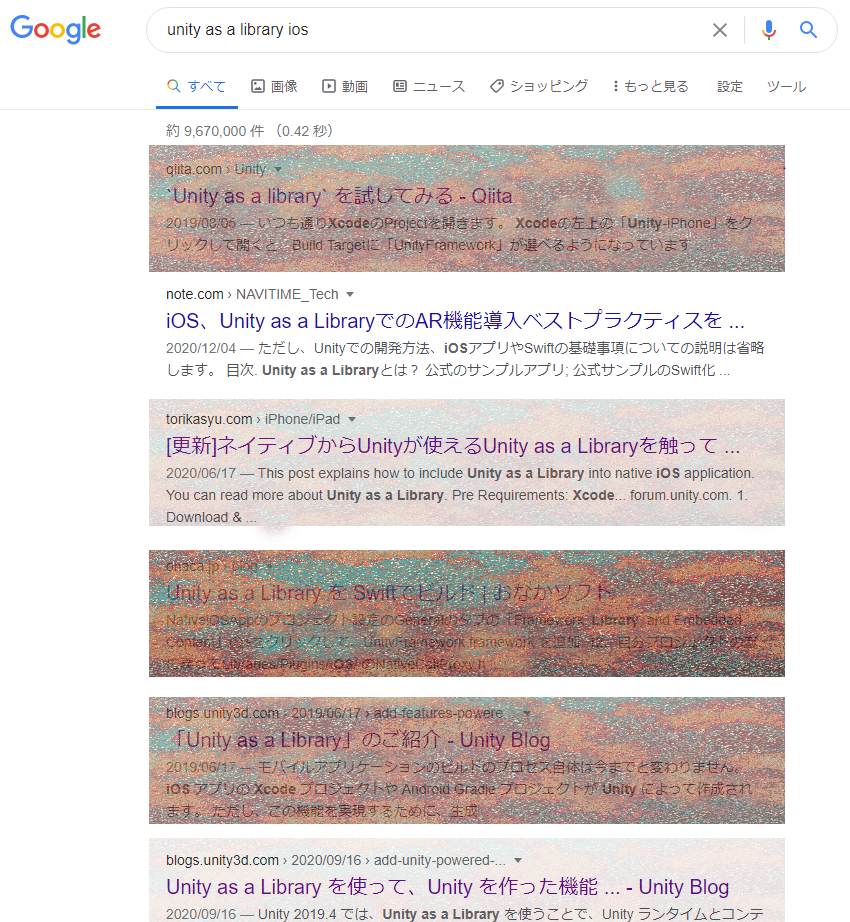
\includegraphics[width=60mm]{images/iron-russet1.png}}
    \end{center}
    \caption{金属のさびをイメージした視覚化1}
    \label{fig:ver-russet1}
  \end{minipage}
  \begin{minipage}{0.5\hsize}
    \begin{center}
      \fbox{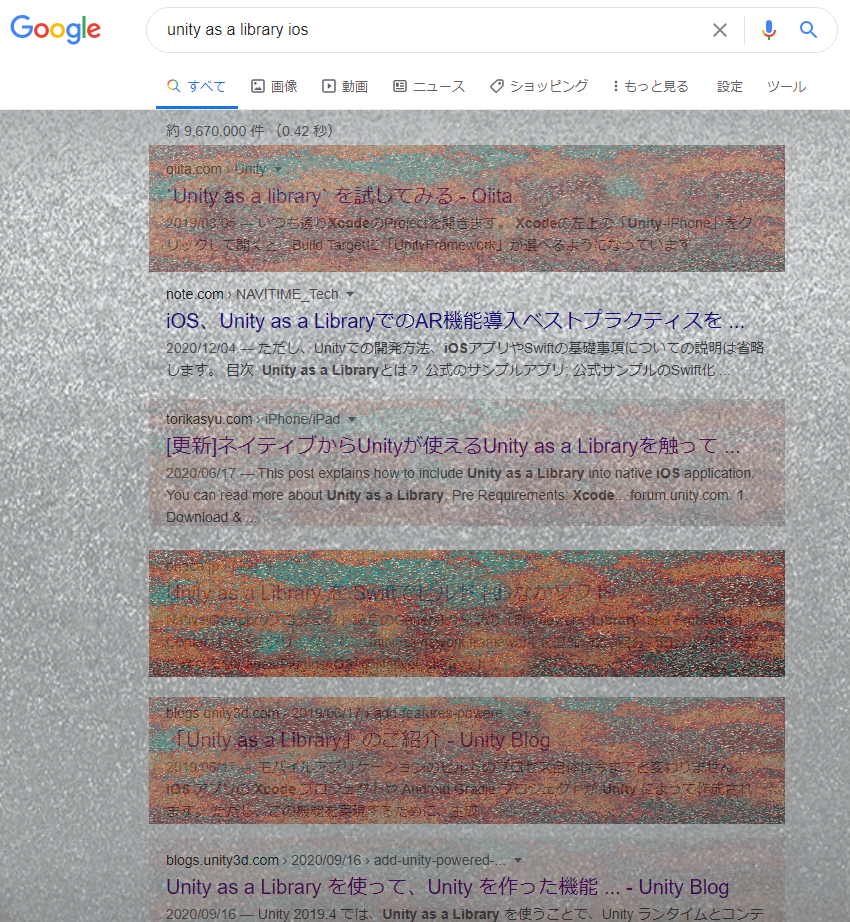
\includegraphics[width=60mm]{images/iron-russet2.png}}
    \end{center}
    \caption{金属のさびをイメージした視覚化2}
    \label{fig:ver-russet2}
  \end{minipage}
\end{figure}

図\ref{fig:ver-russet1}は\ref{subsec:ver-tex-sheet}の方法を錆びた金属のテクスチャを用いて行ったものである.

また,図\ref{fig:ver-russet2}は,図\ref{fig:ver-russet1}に加えて,背景に金属のテクスチャを適用することで,錆びた金属のテクスチャがなじむようにしたものある.

\ref{subsec:ver-tex-sheet}と比べて古い情報が強調されているが,金属に存在する光沢や凹凸,錆によって文字が読みにくくなっており不便である.金属のテクスチャを使う場合は,文字のフォントにも工夫する必要がある.

\subsection{色による変化}
\label{sec:ver-color}

\subsubsection{背景色の変化}
\label{subsec:ver-col-cor}

実世界のモノが腐食するイメージを参考に背景色を変化させる.

\begin{figure}[htbp]
  \begin{minipage}{0.5\hsize}
    \begin{center}
      \fbox{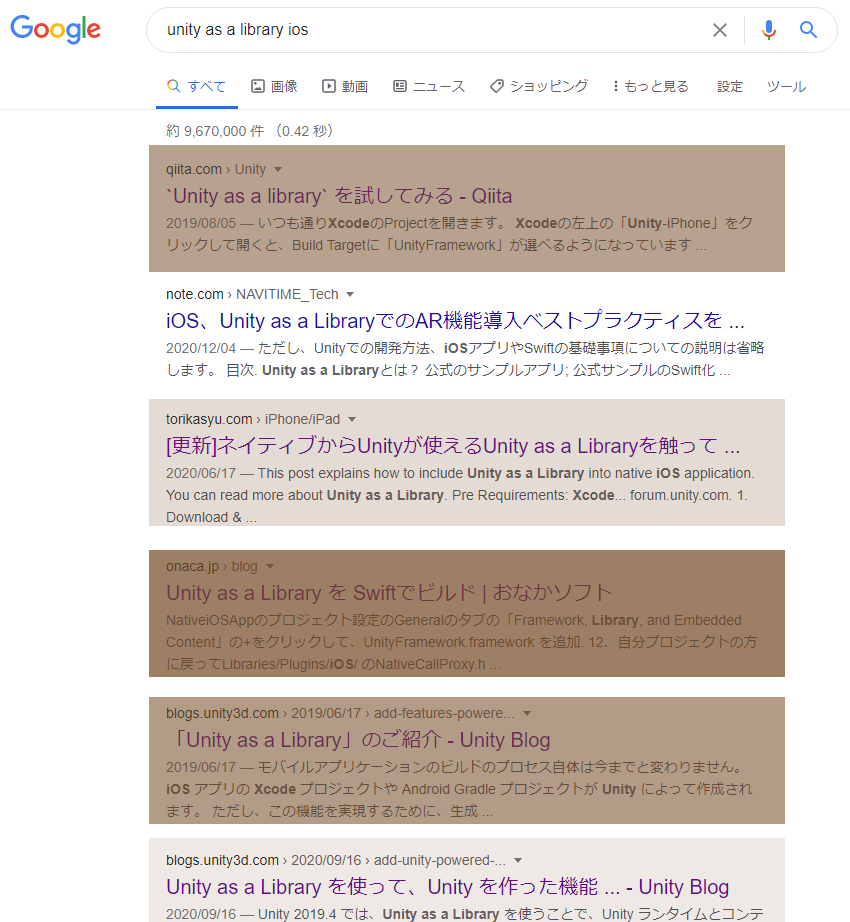
\includegraphics[width=60mm]{images/corrosion1.png}}
    \end{center}
    \caption{腐食をイメージした視覚化1}
    \label{fig:ver-corrosion1}
  \end{minipage}
  \begin{minipage}{0.5\hsize}
    \begin{center}
      \fbox{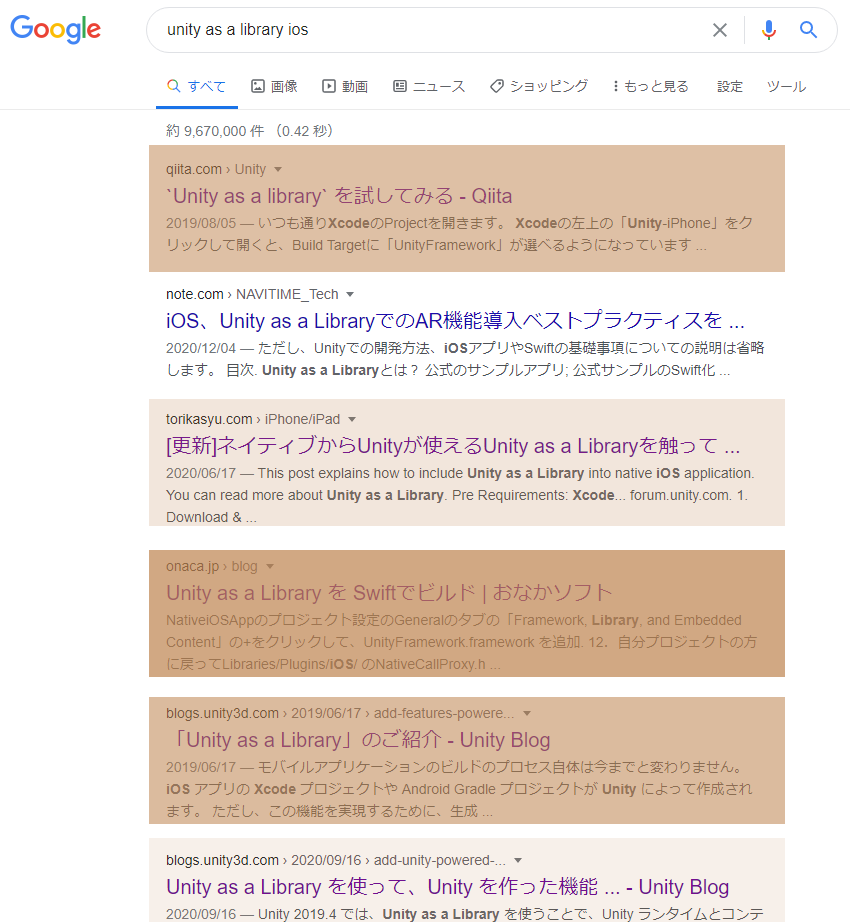
\includegraphics[width=60mm]{images/corrosion2.png}}
    \end{center}
    \caption{腐食をイメージした視覚化2}
    \label{fig:ver-corrosion2}
  \end{minipage}
\end{figure}

モノの腐食を参考にした,図\ref{fig:ver-corrosion1},図\ref{fig:ver-corrosion2}は,暗い茶色や赤茶色をベースにして鮮度が良いと白に近づくように各検索結果の背景色を変化させた.

コンセプトとしては\ref{sec:ver-texture}で検証した二つと近いが,こちらの方が単色での変化なので元の白い背景に対して不自然さが少ない.しかし,色の変化が鮮度を示していることを認識しにくい.

永井らの実験によれば,画像全体に対し黄色方向への色変化やムラを加えることが,古さを感じさせる手法として有効\cite{fading}とあるが,検索結果一覧では元が文章であるためなのか変化が乏しい.

適応する色の選定部分において議論の余地がある.

\subsubsection{インクの劣化}
\label{subsec:ver-col-ink}

紙に書いた文字のインクは時間経過によって劣化していく.そういった変化を参考に,文字の色を変化させる.

\begin{figure}[htbp]
  \begin{minipage}{0.5\hsize}
    \begin{center}
      \fbox{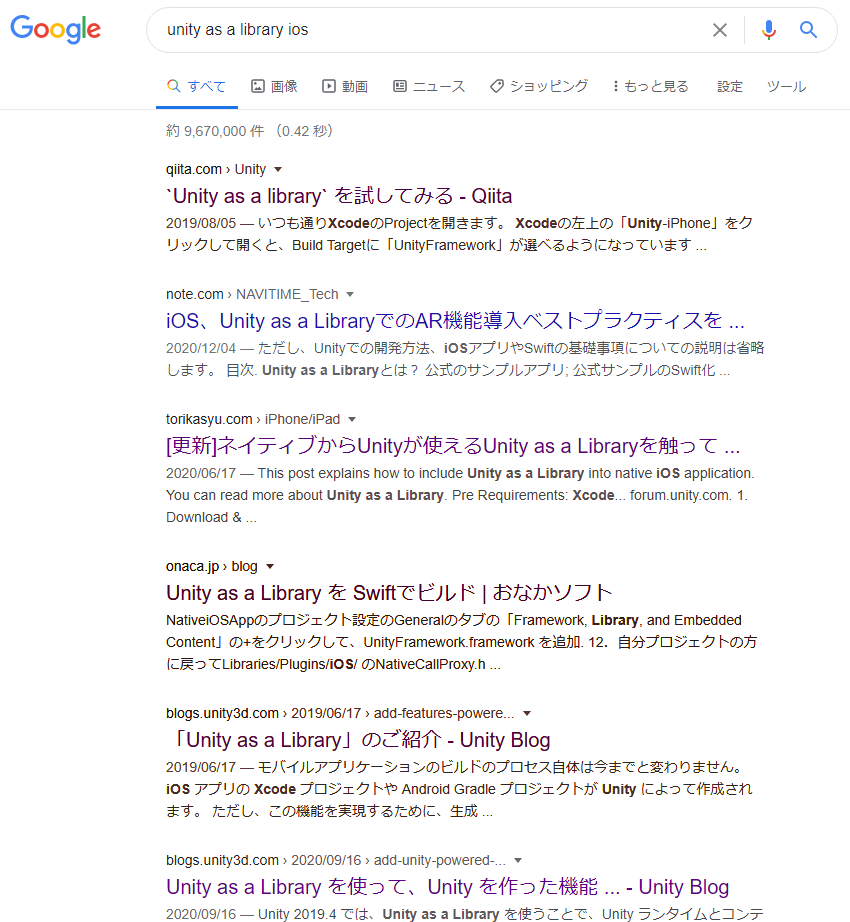
\includegraphics[width=60mm]{images/ink1.png}}
    \end{center}
    \caption{インクの劣化をイメージした視覚化1}
    \label{fig:ver-ink1}
  \end{minipage}
  \begin{minipage}{0.5\hsize}
    \begin{center}
      \fbox{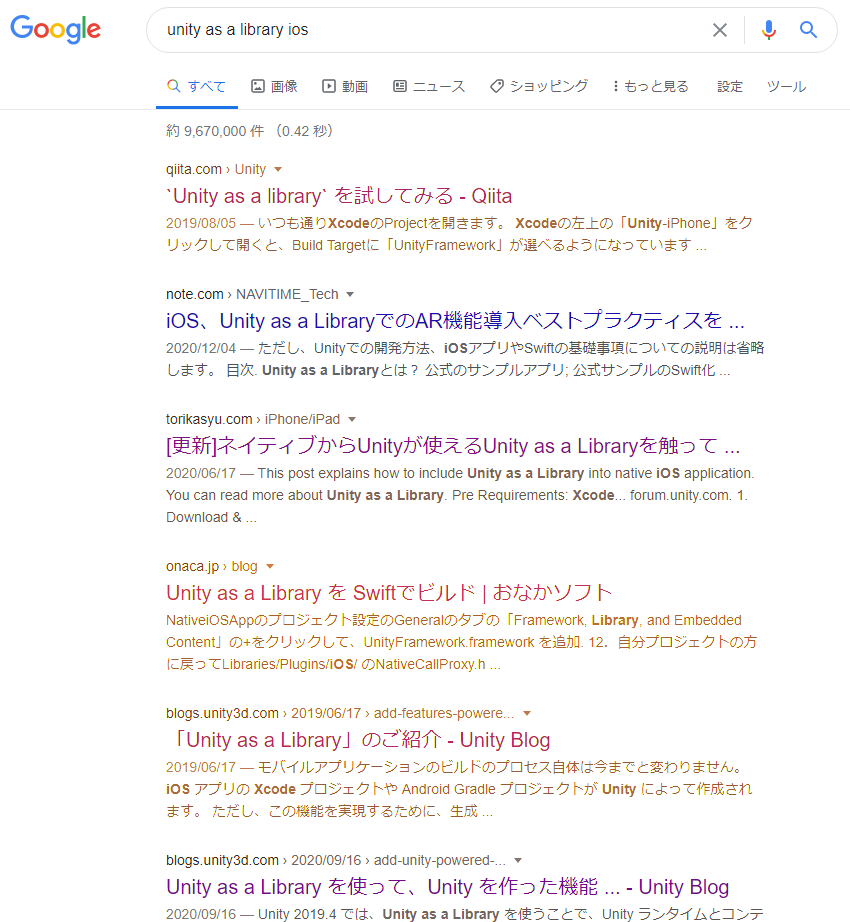
\includegraphics[width=60mm]{images/ink2.png}}
    \end{center}
    \caption{インクの劣化をイメージした視覚化2}
    \label{fig:ver-ink2}
  \end{minipage}
\end{figure}

\ref{subsec:ver-col-cor}と同様に,図\ref{fig:ver-ink1}では,情報の鮮度に応じて文字の色が焦げ茶色に近づくように変化させた.

また,図\ref{fig:ver-ink2}は,文字の色が背景色に薄まるように変化を加えている.

図\ref{fig:ver-ink1}は,視覚化による変化が目立たなかった.これではユーザに情報の鮮度を認識させるという目的が果たせていない.

図\ref{fig:ver-ink2}は,古い印象を与えることには成功している.しかし,各情報同士の鮮度の違いを認識しづらい.

インクの劣化を参考にした視覚化は,段階的な変化の表現に適していないと考える.

\subsection{文字の消失による変化}
\label{sec:ver-character}

\subsubsection{透明化}
\label{subsec:ver-chr-trp}

実世界のモノは時間経過によって風化していく.その消失していくさまをイメージして,各項目の不透明度を変更する.

\begin{figure}[htbp]
  \begin{center}
    \fbox{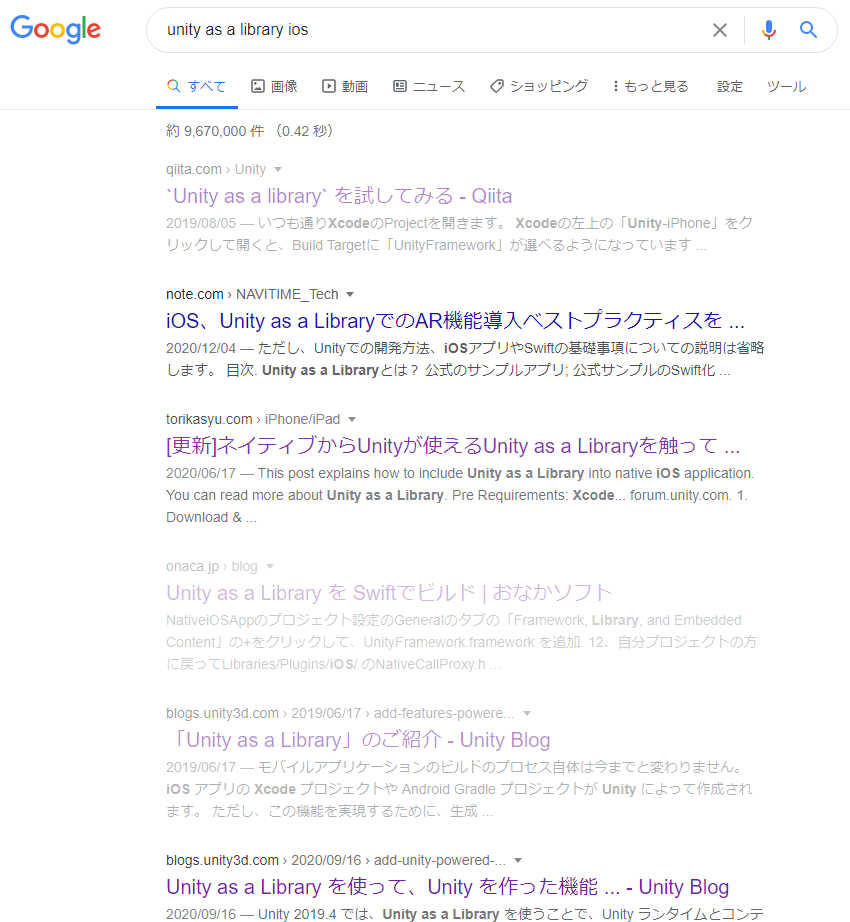
\includegraphics[width=60mm]{images/transparence.png}}
  \end{center}
  \caption{不透明度を変更した視覚化}
  \label{fig:ver-transparence}
\end{figure}

図\ref{fig:ver-transparence}は,各情報ごとに古ければ古いほど不透明度が下がっていくようにしている.

元の検索画面に対して微小な変更のみを加えているため,不自然な点が少ない.また,段階的な変化を感じやすく,時間経過を簡単に認識できる.

しかし「薄い(不透明度が低い)=古い」という結びつけが弱いため,鮮度を表しているという認識をユーザに与えられるか疑問がある.

\subsection{滲みの利用}
\label{subsec:ver-chr-bld}

紙にインクを垂らすと時間が経つに連れてインクは滲んでいく.そのイメージを参考に,文字を滲ませる.

\begin{figure}[htbp]
  \begin{center}
    \fbox{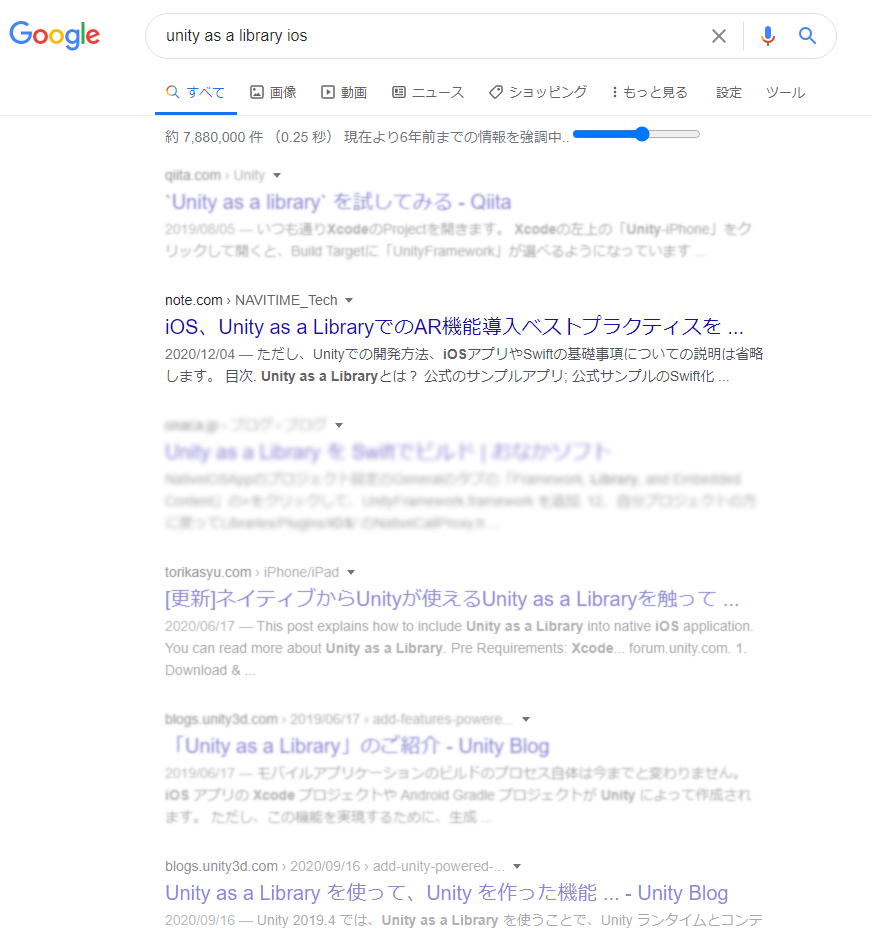
\includegraphics[width=60mm]{images/bleeding.png}}
  \end{center}
  \caption{インクの滲みをイメージした視覚化}
  \label{fig:ver-bleeding}
\end{figure}

図\ref{fig:ver-bleeding}は,各情報ごとに古ければ古いほどで文字が滲んでいくようにしている.

\ref{subsec:ver-chr-trp}のように元の背景とよくなじみ,段階的な変化が感じやすい.加えて,古い情報が読みにくくなるため,新しい情報に目が行きやすくなる効果も期待できる.

しかし,滲んでいるから古い情報だという結びつけは弱いように思われる.

\subsubsection{虫食い}
\label{subsec:ver-chr-wh}

古い書物などは紙自体の経年劣化の他にシミなどによる虫食いで欠落が見られる.そういった劣化の仕方を参考に文字に変化を加える.

\begin{figure}[htbp]
  \begin{minipage}{0.5\hsize}
    \begin{center}
      \fbox{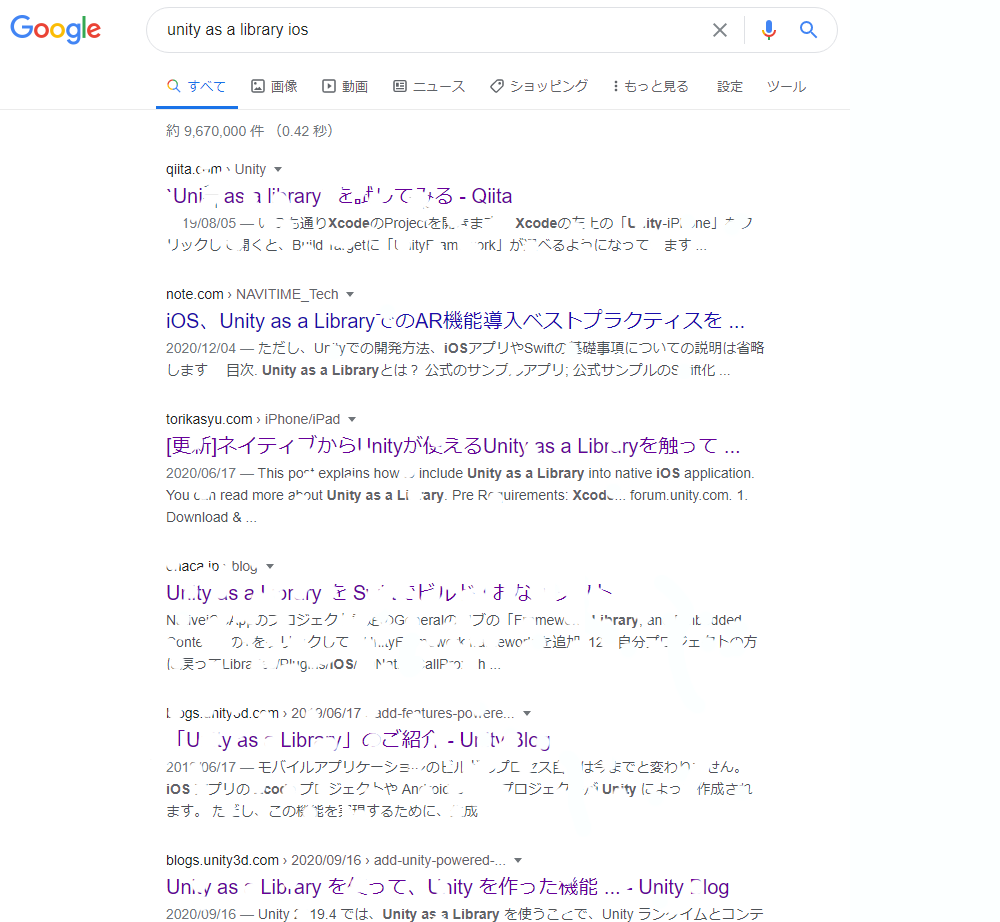
\includegraphics[width=60mm]{images/wormhole1.png}}
    \end{center}
    \caption{虫食いをイメージした視覚化1}
    \label{fig:ver-wormhole1}
  \end{minipage}
  \begin{minipage}{0.5\hsize}
    \begin{center}
      \fbox{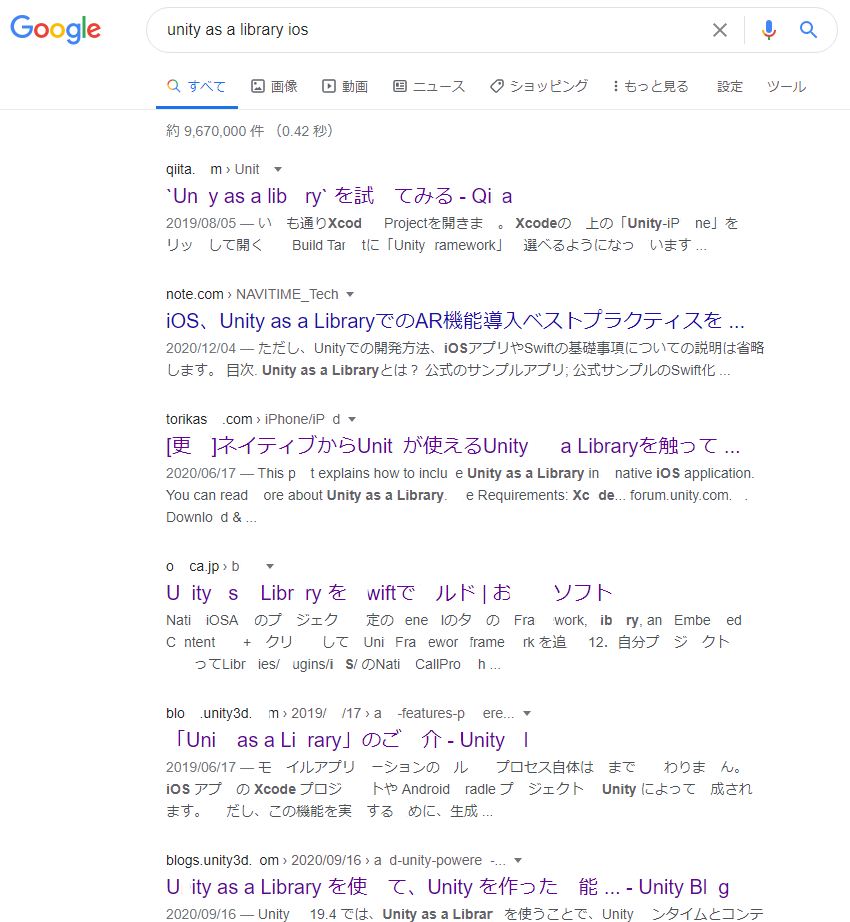
\includegraphics[width=60mm]{images/wormhole2.png}}
    \end{center}
    \caption{虫食いをイメージした視覚化2}
    \label{fig:ver-wormhole2}
  \end{minipage}
\end{figure}

図\ref{fig:ver-wormhole1}は実際に虫に食われた紙をイメージして,古ければより文字の一部分が欠損するように視覚化をしている.

図\ref{fig:ver-wormhole2}は文章の虫食いをイメージして,古ければ古いほど多くの文字が欠落するように視覚化をしている.

どちらも情報の鮮度に応じた変化の差を設けるのが難しく,\ref{subsec:ver-col-ink}の視覚化と同様,鮮度に応じた段階的な変化は感じられない.

しかし,古い情報を目立たせない効果は十分にあると考える.

\subsection{フォントによる変化}
\label{sec:ver-font}

\subsubsection{異なる書体の利用}
\label{subsec:ver-fnt-stl}

時代が進むごとに文字の書体も変化して\footnote{5分で学ぶフォントの歴史500年|時代背景とタイポグラフィ, https://note.com/smartcamp-design/n/n2740a3b72be9}おり,書体だけで時代を感じることもできる.つまり,書体で時間の経過を表すことも可能だと推測する.

そこで,古い情報は古そうだと感じられる書体を,新しい情報は新しそうだと感じられる書体を用いて記述することで鮮度の違いを表現する.

\begin{figure}[htbp]
  \begin{center}
    \fbox{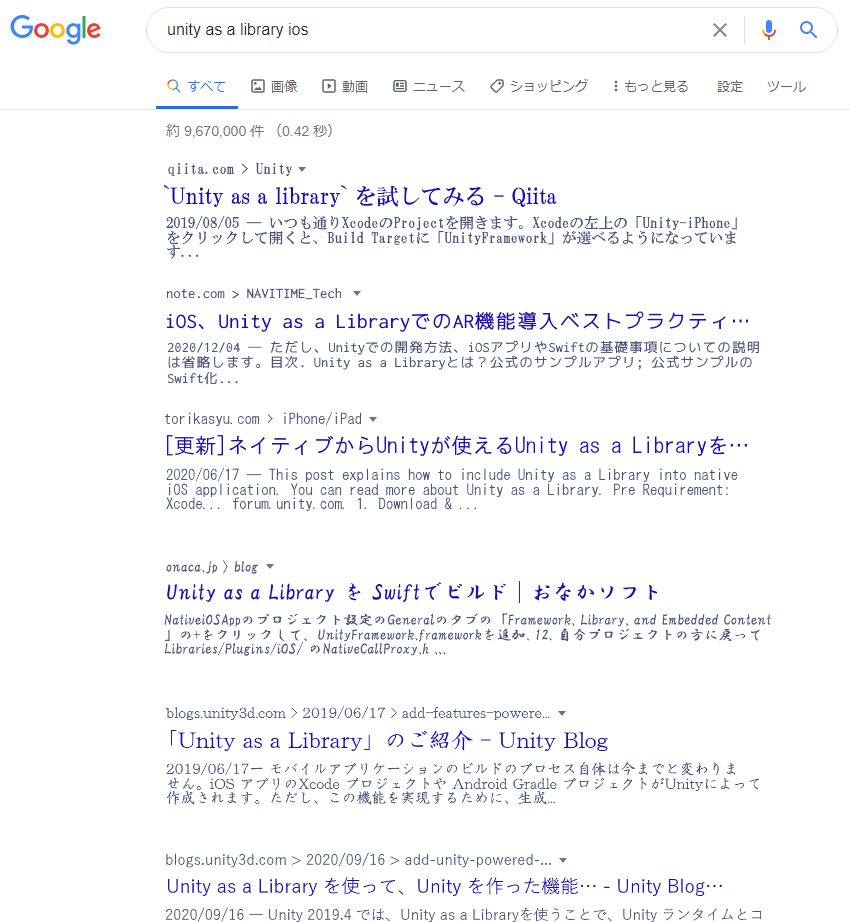
\includegraphics[width=60mm]{images/font-style.png}}
  \end{center}
  \caption{書体の変化による視覚化}
  \label{fig:ver-style}
\end{figure}

図\ref{fig:ver-style}は各情報ごとに,古いものは楷書体や行書体のフォントを使い,新しいものはゴシック体などを使うように変更したものである.

画像を作成する際に,以下の二つの問題点が見つかった.

\begin{itemize}
  \item フォントの選定が難しい
  \item 人によってフォントに対する印象が違う
\end{itemize}

多数存在するフォントの中から鮮度に合わせたフォントをピックアップするのは難しい.また,フォントを選定した人間の感覚では完璧であっても,人によってフォントに対する印象が違うため,第三者が利用する場合に鮮度を認識できない可能性がある.

\subsection{ドットフォントの利用}
\label{subsec:ver-fnt-dot}

古い電子機器の画面ではピクセル数の関係からドットフォントが使用されていたり,古さを演出するために意図的にドットフォントを使うこともある.

そこで,粒度の違うドットフォントを用いて情報の鮮度を表現する.

\begin{figure}[htbp]
  \begin{center}
    \fbox{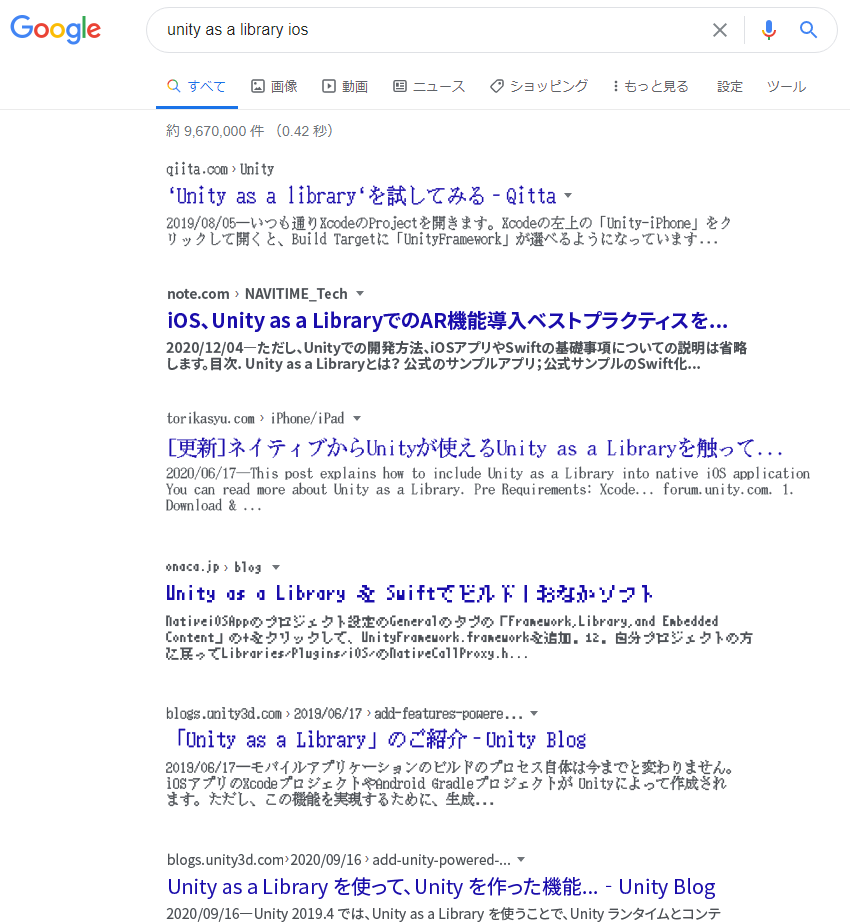
\includegraphics[width=60mm]{images/font-dot.png}}
  \end{center}
  \caption{ドットフォントの粒度の変化による視覚化}
  \label{fig:ver-dot}
\end{figure}

図\ref{fig:ver-dot}は,古ければ古いほど粒度の荒いドットフォントを使用している.

予測では鮮度の段階ごとの変化を感じやすいと思われたが,古い印象よりも各サイトごとの特色だという印象の方が強かった.

これは各ドットフォントがそれぞれ特徴的で,段階的な変化を感じさせなかったためだと推測される.
